
\فصل{روش پیشنهادی}
\label{فصل:روش پیشنهادی}

\قسمت {چارچوب کلی}
\label{قسمت:چارچوب کلی}
چارچوب کلی روش پیشنهادی ارائه‌شده بدین صورت است که در ابتدا گردش‌های کاری میان میکروسرویس‌های تشکیل‌دهنده‌ی نرم‎افزار را با استفاده از زبان یاول مدل می‎کنیم. سپس این مدل‌ها را بر اساس روش ترجمه‌ای اثبات شده، به یک توصیف صوری در زبان الوی ترجمه می‌کنیم. بعد از آن بر روی توصیف صوری از میکروسرویس‌ها و ارتباطات آن‌ها تحلیل‌هایی صوری به زبان الوی انجام می‌دهیم تا وجود موقعیت‌های ناخواسته و غیرمجاز در اجرای گردش کاری نرم‌افزار را بررسی کنیم. به علاوه با استفاده از توصیفات صوری مذکور و بر اساس معیار پوشش گزاره‌ی فعال محدود، نیازمندی‌های آزمون و سپس برای برآورده کردن هر یک از نیازمندی‌های آزمون موارد آزمون را تولید می‌کنیم و در انتها موارد آزمون به دست آمده که آن‌ها نیز توصیفاتی صوری هستند را به توصیف اصلی اضافه می‌کنیم؛ سعی می‌کنیم یک نمونه از توصیف به‌دست آمده بسازیم، در صورت سازگار ماندن توصیف، این نمونه به دست می‌آید و موفقیت‌آمیز بودن اجرای آزمون را نشان می‌دهد. 

روند کلی روش ارائه‌شده در شکل~\رجوع{شکل: روند کلی روش ارائه‌شده} آورده شده است.
\شروع{شکل}[t]
\centerimg{method-flow}{16cm}
\vspace{0.3em}
\شرح{روند کلی روش ارائه‌شده}
\برچسب{شکل: روند کلی روش ارائه‌شده}
\پایان{شکل}

تمام این روند، پس از مدل‌سازی میکروسرویس‌ها در زبان یاول توسط طراحان نرم‎افزار، تا ایجاد موارد آزمون و اعمال آن‌ها بر روی مدل صوری به صورت خودکار در ابزار مدل‌سازی یاول انجام می‌شود.

در ادامه به تشریح گام‌های ذکر شده در روش پیشنهادی می‌پردازیم. اما برای روشن‌تر شدن این روش یک نمونه‌‌ی برگرفته‌شده از یک سیستم نرم‌افزاری با معماری میکروسرویس در دنیای واقع را می‌آوریم و در هر گام، روش تشریحی خود را بر روی این نمونه‌ی واقعی اِعمال می‌کنیم. 




\قسمت{مدل‌سازی سیستم‌های پیچیده با معماری میکروسرویس با یاول}
امروزه خیلی از برنامه‎ها شامل مجموعه‌ای از سرویس‌ها هستند هر میکروسرویس به طور مستقل توسعه یافته، مستقر و مدیریت می‌شود. 
همکاری میکروسرویس‌ها با یکدیگر هدف برنامه را محقق می‌کند؛ هماهنگی و تعامل میان میکروسرویس‌ها با به کارگیری یکی از دو رویکرد ارکستراسیون یا  موزون انجام می‌شود.
به دلیل ذات غیرمتمرکز میکروسرویس‌ها به نظر می‌رسد استفاده از رویکرد موزون برای ترکیب\پاورقی{Compostion} آن‌ها مناسب تر باشد. 
در سبک موزون، هر میکروسرویس به طور مستقل کار می‌کند، در حالی که، در ارکستراسیون، یک کنترل‌کننده\پاورقی{Controller} وجود دارد که تعاملات سرویس را هماهنگ می‌کند\مرجع{valderas2020}\مرجع{nadeem2022}.

ما روشی برای آزمون هر دو این سبک‌ها ارائه می‌کنیم اما نمونه‌ای که برای روشن‌تر شدن موضوع استفاده شده‌است از رویکرد ارکستراسیون برای ساختن معماری میکروسرویسی خود استفاده می‌کند. 

استفاده از زبان‌ مدل‌سازی یاول که یک زبان مدیریت فراروند کسب و کاری است یکی از رویکردها برای مدل‌سازی از این تعاملات بین میکروسرویس‎ها در یک برنامه‌ی پیچیده است\مرجع{valderas2020}.

در روش پیشنهادی، ابتدا یک برنامه با استفاده از یاول مدل می‌شود، میکروسرویس‌ها واحد‌های مستقلی هستند که هر کدام جزئی از کل کار برنامه را بر عهده دارند و گردش کار بین میکروسرویس‌ها معمولا با رد و بدل شدن پیام بین آن‌ها انجام می‌پذیرد \مرجع{heorhiadi2016}،
 در سبک موزون این ارتباط بدون واسطه و مستقیم انجام می‌شود. 
 
 در یاول کوچک‌ترین واحدهای کاری مستقل، وظایف هستند و می‌توان آن‌ها را معادل میکروسرویس‌ها در یک برنامه در نظر گرفت. 
 همچنین در یاول ارتباط میان وظایف با جریان‌ها برقرار می‌شوند، \مرجع{yawlbook} می‌توان برای نمایش ارسال پیام‌ها میان میکروسرویس‌ها از جریان‌ها استفاده کرد. 
 از انشعاب‌ها و اتصال‌ها برای هدایت گردش کار در یاول استفاده می‌شود، در آن‌ها با توجه به متغیر‌های ورودی و خروجی و شروط اعمال شده بر روی آن‌ها گردش کار توسط وظایف هدایت می‌شود. 
 مقادیر متغیرها در برنامه را خروجی میکروسرویس‌ها تعیین می‌کنند و جریان کنترل در برنامه با توجه به خروجی هر میکروسرویس بین آن‌ها گردش می‌کند. 

  \قسمت{خودکارسازی ترجمه‌ی مدل‌های یاول به الوی}
  
  \زیرقسمت{توصیف مدل‌ها در زبان الوی}
  
برای ترجمه‌ی مدل‌های یاول به توصیفات صوری در زبان الوی، از روشی که در پژوهش ریواده و همکاران انجام شده است\مرجع{rivadeh2022} استفاده کردیم؛
 در روشی که ریواده و همکاران برای ترجمه ارائه کرده‌اند، ساختار مدل‌ها در یاول به دو بخش ایستا و پویا تقسیم‌بندی شده‌است و برای هر یک از موجودیت\پاورقی{‌Entity}‌ها در هر دسته معادلی در الوی ذکر شده‌است. 
 همچنین برای ویژگی‌های ذاتی مدل‌های گردش کاری در یاول مانند هم‌بند بودن گراف، در الوی حقیقت\پاورقی{fact}‌هایی تعریف شده‌است.
  در نهایت روشی برای ترجمه‌ی مدل‌ها به دست آمده و سپس با نه قضیه نشان داده‌است که ترجمه‌ی به دست آمده از مدل‌های گردش کاری در یاول به زبان الوی کامل و صحیح\پاورقی{sound} هستند.
  
بخش ایستا در مدل‌ها، همان مفاهیم و مولفه‌های موجود در زبان یاول هستند. در پژوهش ریواده این بخش شامل وظیفه\پاورقی{task}، شرط ورودی\پاورقی{input condition}، شرط خروجی\پاورقی{output condition} و شرط است؛ 
برای هر کدام از این مولفه‌ها در الوی یک معادل در قالب نشان\پاورقی{signature} آورده شده است. همچنین رفتار انواع پیوند\پاورقی{join}ها و انشعاب\پاورقی{split}‌ها نیز در قالب حقیقت‌ها بیان شده اند. 
علاوه بر این‌ها بخش ایستا در ترجمه‌ی تولید‌شده شامل تعریف حالت\پاورقی{state} در یک گردش کار نیز می‌شود به تعریف حالت در الوی ترتیب اضافه شده‌است، 
این کار اجازه می‌دهد بتوان تغییر حالت‌ها در زمان را مدل کرد. ترتیب حالت‌ها توسط پودمان کتابخانه util/ordering ارائه می‌شود. این پودمان عمومی است - یعنی می‌تواند به مجموعه‌ای از هر نوع ترتیب بدهد - بنابراین وقتی باز می‌شود باید با یک نوع (در این مورد، حالت) نمونه‌سازی\پاورقی{instantiate} شود\مرجع{alloybook}.

مجموعه‌ی توکن مجموعه‌ای از وظایف یا شرط ورودی یا شرط خروجی است که کاری در آن‌ها در حال انجام است در هر حالت از گردش کار، توکن در یک یا چند وظیفه وجود دارد و با تغییر حالت، در میان وظیفه‌ها جابجا می‌شود. در واقع و تغییر حالت متناظر با تغییر مجموعه‌ی توکن است. 
بخش پویا مرتبط با معماری میکروسرویسی است که در یاول مدل شده است. 

برای ترجمه‌ی مدل تعریف شده به الوی، برای هر وظیفه که معادل یک میکروسرویس است، حقیقت یا حقیقت‌هایی در الوی تعریف می‌کنیم و در آن(ها) ویژگی‌های وظیفه شامل نام، نوع پیوند، نوع انشعاب و جریان‌های خروجی آن را ذکر می‌کنیم؛ 
همچنین مسندهایی که در جریان‌های خروجی وظیفه تعریف شده‌اند را نیز بسته به نوع انشعاب، در گزاره‌های شرطی ذکر می‌کنیم. 
بخش‌ پویا در واقع نشان‌دهنده‌ی میکروسرویس‌ها و نحوه‌ی ارتباط آن‌ها با یکدیگر هستند و شامل وظیفه و جریان‌های بین آن‌ها می‌شود.
 
به روش ریواده و همکاران برای ترجمه‌ی مدل‌های یاول به الوی موارد جدیدی اضافه کردیم که در ادامه به آن‌ها می‌پردازیم؛ در ترجمه‌ای که از مدل‌های یاول تولید می‌کنیم، شامل توصیف ناحیه‌ی لغو در بخش ایستا نیز می‌باشد، 
همچنین در تعریف وظیفه‌ها نیز مجموعه‌ی وظیفه‌هایی که در ناحیه‌ی لغو آن وظیفه وجود دارند تعریف می‌شود. 
متغیرهای موجود در مدل گردش کاری که شامل ورودی خروجی وظیفه‌ها و معادل ورودی و خروجی میکروسرویس‌ها هستند، در تعریف حالت ذکر می‌شوند. 
مقادیر متغیرها در هر حالت امکان تغییر دارند و رفتار میکروسرویس‌ها در هر حالت بسته به مقدار متغیرها و شرایط درونی میکروسرویس می‌تواند تغییر کند.


\زیرقسمت{جای‌گذاری روش در ابزار ویرایش یاول}
روش پیشنهادی گفته شده را در ابزار ویرایشگر یاول جاسازی کردیم و کار ترجمه در این ابزار به صورت خودکار انجام می‌شود و در خروجی به طراح نرم‌افزار نمایش داده می‌شود. برای تولید ترجمه به این صورت عمل می‌کنیم: قسمت‌های ایستا به صورت ثابت و ایستا به ترجمه اضافه می‌شوند اما برای ترجمه‌ی خودکار مولفه‌های متغیر در مدل‌ها، پیش‌‎پردازشی بر روی فرم استاندارد ذخیره‌شده‌ی مدل‌ یاول انجام می‌دهیم و سپس با روشی هر کدام از مولفه‌های پویا را تجزیه و تحلیل می‌کنیم و آن‌ها را به اشیائی از کلاس‌های تعریف شده در زبان جاوا تبدیل می‌کنیم و سپس در انتهای کار ترجمه از هر کدام از آن اشیاء، توصیف آن‌ها را به زبان الوی پرس و جو می‌کنیم و سپس آن‌ها را تجمیع و به قسمت‌های ایستای توصیف اضافه می‎کنیم. در نهایت، توصیف به دست آمده شامل تعاریف اجزای ایستای مدل‌ها که شامل انواع پیوندها و انشعاب‌ها و همچنین تعاریف وظیفه و شرط ورودی و شرط خروجی است.


\قسمت{تحلیل صوری مدل‌ها}
با توجه به اینکه گردش‌های کاری میکروسرویس‌های استقراریافته، ممکن است برای مدت طولانی به صورت مداوم اجرا شوند و ممکن است اقدامات زیادی انجام دهند که به سادگی قابل بازگرداندن نیستند، تشخیص خطاها در زمان طراحی بسیار می‎تواند کمک‌کننده باشد. هنگامی که از تحلیل گردش کار صحبت می‌کنیم در واقع به این می‌پردازیم که آیا یک گردش کار رفتارهای مطلوب خاصی را نشان می‌دهد یا خیر. 

پژوهش‌های قبلی زیادی وجود دارد که بر روی تحلیل‌های گردش کار انجام شده‌اند مانند \مرجع{alast1997} که در آن از تکنیک‌های تحلیل شبکه‌ی پتری برای تشخیص درست بودن یا نبودن شبکه گردش کار استفاده می‌شود. اما ضعف آن‌ها در این است که، نتایج پژوهش اشاره‌شده به‌ راحتی قابل اعمال به برخی موقعیت‌ها نیستند. موقعیت‌هایی که در آن زبان‌هایی درگیر هستند که از مفاهیمی مانند منطقه‌ی لغو و پیوند از نوع ``یا'' استفاده می‌کنند. این ضعف به این دلیل است که این مفاهیم را نمی‌توان به راحتی از طریق شبکه‌های پتری بیان کرد. در پژوهش \مرجع{analysis2006} سعی شده است تا روشی بر مبنای شبکه‌های بازنشانی ارائه شود تا این ضعف را پوشش دهد. ما نیز در این بخش به تحلیل‌هایی که با استفاده از روش‌های صوری بر روی مدل گردش کاری در میکروسرویس‌ها انجام می‌دهیم، می‌پردازیم. 

تحلیل‌های که در ادامه می‌آیند، با بررسی درستی اظهار در الوی انجام می‌شود به این صورت که یک اظهار به کل تعریف گردش کاری افزوده می‌شود و سپس توصیف حاصل‌شده را به موتور الوی می‌دهیم. اظهارها به صورت کلی به این فرمت نوشته می‌شوند که "در هیچ نمونه‌ای از توصیف موجود حالت غیرمجاز وجود ندارد" اگر موتور الوی بتواند مثال نقضی برای این اظهار پیدا کند، پیدا شدن نمونه‌ای که این اظهار را نقض کند، در کاربرد ما به منزله‌ی وجود حالتی غیرمجاز است که ساختار گردش کاری باعث پیدایش آن شده است.

\شروع{فقرات}
\فقره بررسی پیوند از نوع "یا" در حلقه: 

بنا بر تعریف، این وضعیت که یک وظیفه که دارای پیوند از نوع "یا" است در حلقه قرار گیرد، غیرمجاز است؛ در این حالت، وظیفه‌ای که دارای پیوند از نوع "یا" است منتظر مشخص شدن وضعیت شاخه‌ی ورودی خود است در حالی که مشخص شدن وضعیت شاخه‌ی ورودی به خروجی همین وظیفه بستگی دارد و در نتیجه گردش کار دچار نوعی بن‌بست می‌شود. برای تشخیص این حالت غیرمجاز در روش پیشنهادی خود، تحلیلی را ارائه کردیم که با بررسی ساختار گردش کاری ورودی که آیا وظیفه‌ای باعث ایجاد این حالت غیرمجاز می‌شود یا خیر.

همان‌طور که در بالاتر شرح داده‌شد، این تحلیل با افزودن یک اظهار و سپس بررسی آن در توصیف انجام‌ می‌شود. اظهار به صورت زیر توصیف می‌شود. 



\شروع{شکل}[H]
\raggedright
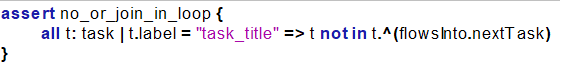
\includegraphics[width=9cm]{no-or-join-in-loop}
\vspace{0.5em}
\برچسب{شکل: اظهار تولیدشده برای اطمینان از عدم وجود پیوند از نوع ``یا'' در حلقه}
\پایان{شکل}




\فقره قابل دسترس بودن وظایف:

میکروسرویس‌هایی که در معماری نرم‌افزار استفاده شده‌اند مسئولیت انجام قسمتی از خدمت را به عهده دارند در نتیجه در طول اجرای نرم‌افزار زمانی وجود خواهد داشت که هر میکروسرویس در حال انجام وظیفه‌ای است که به عهده دارد، اگر میکروسرویسی در جریان کنترل نرم‌افزار قابل دسترسی نباشد وجود آن میکروسرویس برای نرم‌افزار غیرضروری است؛ به طوری که گردش کار بدون وجود آن وظیفه‌‌ی غیر قابل دسترس نیز همان رفتاری را نشان می‌دهد که با وجود آن وظیفه دارد.

در این تحلیل، برای هر وظیفه به دنبال این هستیم که در حداقل یک حالت‌ از گردش کار، وظیفه‌ی مورد بررسی، در مجموعه‌ی توکن آن حالت باشد. این تحلیل نیز با افزودن یک اظهار به توصیف و سپس پیدا کردن مثال نقض برای آن توسط موتور الوی انجام‌ می‌شود. اظهار به صورت زیر نوشته می‌شود. 
\شروع{شکل}[H]
\raggedright
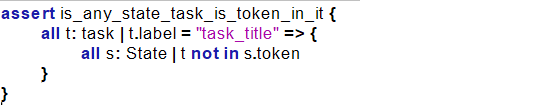
\includegraphics[width=10cm]{reachability-assertion}
\vspace{0.5em}
\برچسب{شکل: اظهار تولیدشده برای اطمینان از قابل دسترس بودن وظیفه}
\پایان{شکل}

اظهار بالا برای تک تک وظایف گردش کاری به صورت متوالی به توصیف گردش کاری افزوده می‌شود و بررسی نیز انجام می‌شود و نتیجه‌ی بررسی آن‌ها به صورت تجمیع شده در خروجی برمی‌گردد.



\فقره منتظر ماندن دو وظیفه با پیوند از نوع "یا" برای یکدیگر:

در این تحلیل، پس از بررسی وجود دو وظیفه با پیوند از نوع "یا" در گردش کاری، با تحلیل ساختار بررسی میکنیم که آیا این دو وظیفه در تصمیم گیری برای جلو رفتن گردش کار در خودشان منتظر یکدیگر هستند یا خیر. چرا که با منتظر بودن این دو وظیفه برای مشخص شدن وضعیت دیگری، وضعیت بن‌بست در گردش کاری رخ می‌دهد که غیرمجاز است.

 این تحلیل نیز با افزودن یک اظهار و سپس بررسی آن در توصیف انجام‌ می‌شود. اظهار را به صورت زیر می‌نویسیم. 
 
 
 
\شروع{شکل}[H]
\raggedright
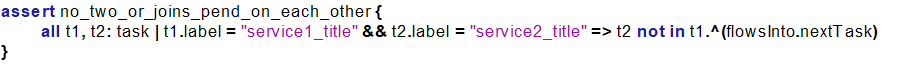
\includegraphics[width=17cm]{two-pending-or-joins-assertion}
\vspace{0.5em}
\برچسب{شکل: اظهار نوشته‌شده برای بررسی منتظر بودن دو پیوند از نوع ``یا''}
\پایان{شکل}




\پایان{فقرات}




\قسمت{ایجاد موارد آزمون و اعمال آن‌ها بر روی مدل}
آزمون نرم افزار یک فرآیند حیاتی است که کیفیت محصولات نرم افزاری را تضمین می‌کند. در روش آزمون ارائه‌شده آزمون‌ها بر اساس معیارهای پوشش گزاره‌ی فعال محدود تولید شده‌اند.

پس از اطمینان از قابل دسترس بودن همه‌ی وظایف و هم‌چنین اطمینان از عدم برخورد با وضعیت‌های غیرمجاز به آزمون گردش‌ کار می‌پردازیم در رویکرد ارائه‌شده، جریان کنترل گردش کار را مورد آزمون قرار می‌دهیم، برای آزمون مدل صوری به زبان الوی، موارد آزمون را در مکان‌هایی که در آن‌ها جریان کنترل تعیین می‌شود، تولید می‌کنیم. 

در یک سیستم نرم‌افزاری با معماری میکروسرویس، هر خدمت یا یک مجموعه خدمت توسط یک میکروسرویس انجام می‎گیرد، پاسخ به درخواست کاربر از نقطه‎ای آغاز می‌شود و سپس گردش کار در میان میکروسرویس‌ها شامل ارتباط بین سرویس‌های مختلف برای تکمیل یک فراروند است. هر میکروسرویس ورودی را از سرویس‌های دیگر دریافت می‌کند، عملکرد خود را انجام می‌دهد و خروجی را به سرویس‌های دیگر می‌فرستد. به عبارتی گردش کار به عملکرد هر سرویس وابسته است و تعیین مسیر در گردش کاری با توجه به ورودی و خروجی‌های سرویس‌ها انجام می‌گیرد. 

مدل‌ گردش کاری میکروسرویس‌ها مدل‌سازی سطح بالایی است و به مدل‌سازی از عملکرد داخلی سرویس‌ها پرداخته نمی‌شود و تنها ارتباط آن‌ها و نحوه‌ی تعیین جریان کنترل در آن مشخص می‌شود. در نتیجه ترجمه‌ی این مدل‌ها نیز به صورت صوری شامل توصیف عملکرد داخلی میکروسرویس‌ها نیست و در آن صرفا به توصیف نحوه‌ی گردش کار و جریان کنترل در سیستم پرداخته می‌شود. جریان کنترل در زبان‌ یاول، به وسیله‌ی پیوند یا انشعاب‌ها از انواع مختلف انجام می‌شود برای این درگاه‌ها بسته به نوع آن‌ها شروطی تعیین می‎شود و تصمیم‌گیری با توجه به این شروط و همچنین نوع درگاه گرفته می‌شود. 
ما برای تولید موارد آزمون مسندهایی که در انشعاب‌ها توسط طراح نوشته می‌شوند را مبنا قرار می‌دهیم. گزاره‌های شرطی موجود در انشعاب‌ها در ترجمه‌ی مدل‌ها به زبان الوی در نظر گرفته می‎شوند و در توصیف وظایف آن‌ها نیز توصیف می‎شوند. با پیش‌پردازش توصیف به دست ‌آمده، انشعاب‌ها را می‌یابیم و سپس مسندهای آن‌ها را برای تولید موارد آزمون استخراج می‌کنیم. 

برای تولید خودکار موارد آزمون به روش پوشش گزاره‌ی فعال محدود پودمانی ساختیم که با ورودی مسند، جفت‌های موارد آزمون را برای پوشش گزاره‌ی فعال محدود تولید می‌کند. 

برای به دست آوردن زوج موارد آزمون بر اساس پوشش گزاره‌ی فعال محدود، نیاز است که گزاره‌های اصلی که ارزش کلی مسند را تعیین می‌کنند بیابیم. نیازمندی آزمون برای هر
 $c_i$
 دو شرط وجود دارد: گزاره‌ی اصلی به ارزش "درست" و به ارزش "نادرست" اطلاق شود. مقادیر انتخاب شده برای گزاره‌های فرعی باید در زمانی که گزاره‌ی اصلی "درست" است با زمانی که گزاره‌ی اصلی  "نادرست" است یکسان باشد\مرجع{alloybook}.
می‌توان با محاسبه‌ی مسند به روش زیر برای یک گزاره‌ی خاص، تعیین ارزش مسند را به ارزش گزاره‌ی اصلی وابسته کرد.
 
$P_a = p_{a=True}\oplus p_{a=False}$\newline
برای تولید زوج موارد آزمون بعد از محاسبه‌ی مسند به صورتی که ارزش آن را گزاره‌ی اصلی تعیین کند، ارزش گزاره اصلی را یک بار برابر با "درست" و یک بار نیز برابر "نادرست" قرار می‌دهیم. برای این که بتوانیم ارزش گزاره‌ی اصلی را برابر "درست" یا "نادرست" قرار بدهیم به گونه‌ای متغیر‌های مورد استفاده در گزاره‌ی شرطی را مقداردهی می‌کنیم تا گزاره ارزش مورد نظر را پیدا کند.
در روشی که برای تولید موارد آزمون استفاده کردیم، ابتدا با تجزیه و تحلیل مسند موجود در جریان خروجی گزاره‌های شرطی تشکیل‌دهنده‌ی مسند و متغیرهای موجود در آن‌ها را را استخراج می‌کنیم و  سپس درخت عبارت منطقی را می‌سازیم. درخت عبارت منطقی درختی دودویی است که برای نشان دادن عبارات منطقی و استدلال‌های منطقی استفاده می‌شود. برگ‌های این درخت همان گزاره‌های شرطی هستند و راس‌های میانی آن عملگرهای منطقی هستند. مسند

$(a \wedge b) \vee c$\newline
 را در نظر بگیرید شکل ~\رجوع{شکل: درخت عبارت منطقی برای گزاره‌های مسند نمونه} نمایان‌گر درخت عبارت منطقی آن است.


\شروع{شکل}[t]
\centerimg{expression-diagram}{8cm}
\vspace{0.5em}
\شرح{درخت عبارت منطقی برای گزاره‌های مسند $(a \wedge b) \vee c$}
\برچسب{شکل: درخت عبارت منطقی برای گزاره‌های مسند نمونه}
\پایان{شکل}
با استفاده درخت عبارت منطقی به ازای همه‌ی $P_i$‌ها عبارت
 
$P_a = p_{a=True}\oplus p_{a=False}$\newline
را محاسبه می‌کنیم، سپس با ثابت نگه‌داشتن ارزش گزاره‌های فرعی ارزش $P_i$ را یک بار برابر "درست" و یک بار برابر "نادرست" قرار می‌دهیم. در انتها با تحلیل گزاره‌ها و تجزیه‌ی آن‌ها به عملگرها و عملوندی تشکیل‌دهنده، مقادیر متغیرها را به گونه‌ای به آن‌ها نسبت می‌دهیم که ارزش مورد نظر برای گزاره حاصل شود.

پس از تولید موارد آزمون، آن‌ها را بر روی توصیف اعمال می‌کنیم. هر یک از موارد آزمون را با زبان الوی به صورت صوری توصیف می‌کنیم، سپس توصیف را به توصیف کلی گردش کار اضافه می‌کنیم و آن را با واسط‌های برنامه‌نویسی کاربردی ابزار تحلیل الوی اجرا می‌کنیم. 

اجرای آزمون‌ها با استفاده از تحلیل‌گر الوی انجام می‌شود و در نتیجه در فضایی کوچک و با حالت‌های محدود‌شده انجام می‌گیرد\مرجع{jackson2019}. در نتیجه نمی‌توان موفقیت اجرای یک آزمون را معادل موفقیت همیشگی برنامه با ورودی‎های مورد آزمون دانست، اما ناموفق بودن آزمون وجود خطا در برنامه با وجود ورودی‌های مورد آزمون را تضمین می‌کند. به همین دلیل استفاده از تحلیل‌گر الوی به قدرت روش ارائه‌شده در تشخیص خطاها در برنامه می‎‌افزاید.

زوج‌های موارد آزمون تولید شده برای مجموعه متغیرهای استفاده شده در عبارات شرطی در هر درگاه تولید می‌شوند. طبق تعریف پوشش گزاره‌ی فعال محدود ارزش هر متغیری که مورد آزمون است، تعیین‌کننده‌ی ارزش کلی مسند است. سازگار بودن توصیفی که از اعمال موارد آزمون به دست می‎آید، به معنی موفق بودن آزمون است.\newline\newline

